\documentclass[journal]{IEEEtran}
\usepackage{cite}
% *** GRAPHICS RELATED PACKAGES ***
%
\ifCLASSINFOpdf
  \usepackage[pdftex]{graphicx}
\fi
%
\usepackage[cmex10]{amsmath}


% *** ALIGNMENT PACKAGES ***
%
\usepackage{array}
\usepackage{fixltx2e}

\usepackage{stfloats}
% LaTeX2e). It also provides a command:
\fnbelowfloat

\usepackage{booktabs}
\usepackage{amssymb}
\usepackage{amsmath}
\usepackage{pgf}
\usepackage{tikz}
\usetikzlibrary{arrows,positioning}
%\usetikzlibrary{arrows.meta}
\usepackage{url}
\usepackage{color}
\usepackage{graphicx}
\usepackage{xspace}
\newcommand*{\eg}{e.g.\@\xspace}
\newcommand*{\ie}{i.e.\@\xspace}
\newcommand*{\vs}{vs.\@\xspace}

% correct bad hyphenation here
\hyphenation{wave-let}

\usepackage{color}
\newcommand{\vl}[1]{\textcolor{orange}{Vincent : #1}}
\newcommand{\gl}[1]{\textcolor{red}{Gr\'egoire : #1}}
\newcommand{\ja}[1]{\textcolor{magenta}{Joakim : #1}}
\newcommand{\ml}[1]{\textcolor{blue}{ Mathieu : #1}}



\begin{document}
%
% paper title
% can use linebreaks \\ within to get better formatting as desired
% Do not put math or special symbols in the title.
%\title{An evaluation framework for event detection using a morphological model of acoustic scenes}
\title{Object-based Auditory Scenes Similarity Retrieval and Classification With Wavelet Scattering}

\author{Vincent Lostanlen\thanks{This work is supported by the ERC InvariantClass grant 320959.}, Gr\'egoire Lafay, Joakim And\'en, and Mathieu Lagrange}


% make the title area
\maketitle

% As a general rule, do not put math, special symbols or citations
% in the abstract or keywords.
\begin{abstract}

This paper introduces a generic hierarchical modeling of acoustic scenes using the wavelet scattering features for time spans below the second and object-based segmentation for larger time spans that effectively model the scene. 

Application of the proposed approach to the acoustic scene similarity retrieval and acoustic scene classification tasks on publicly available datasets and state-of-the-art classifier demonstrates its potential. More precisely, features derived from the scattering transform consistently outperform Mel-frequency cepstral coefficients (MFCCs) for both tasks. 

Representing the scene at larger time scale as a set of examplars of coherent segments is an effective approach for similarity retrieval as it allows the retrieval system to focus on discriminative features. This benefit is reduced in supervised settings, probably because much of the discriminability potential of the approach is already learned by the classifier.

\end{abstract}

% Note that keywords are not normally used for peerreview paper.
\begin{IEEEkeywords}
Acoustic scene classification, acoustic scene segmentation.
\end{IEEEkeywords}

% For peer review papers, you can put extra information on the cover
% page as needed:
% \ifCLASSOPTIONpeerreview
% \begin{center} \bfseries EDICS Category: 3-BBND \end{center}
% \fi
%
% For peerreview papers, this IEEEtran command inserts a page break and
% creates the second title. It will be ignored for other modes.
\IEEEpeerreviewmaketitle

\section{Introduction}

\IEEEPARstart{T}{he} amount of audio data recorded from our sonic environment has considerably grown over the past decades.
In order to measure the modification of animal biodiversity due to human activity or climate change, the research field of eco-acoustics \cite{ECOACOUSTICS2014, krause} is recently undertaking the massive deployment of acoustic sensors throughout the world \cite{warren2006urban, NessSST13, stowell13a, stowell13b}.
In addition, some recent works demonstrate the interest of acoustic monitoring for the characterization of human pleasantness in urban areas \cite{lafayPartI, guyot2005urban, ricciardi2015sound} as well as the prediction of annoyance due to traffic \cite{gloaguen}.
Because they bear a strong societal impact and raise many scientific challenges, we believe that these case studies are of interest for the signal processing community.

Unfortunately, the field of signal-based ecoacoustics is still in infancy.
As a consequence, very few well built datasets are readily available for evaluation purposes.
A closely related field of investigation, which is relatively more mature, is the classification of acoustic scenes whose aim is to predict labels by processing audio data.
Despite being narrower in terms of range of applications, it has the advantage of being rooted by numerous works in cognitive psychology on categorization \cite{dubois2006cognitive, maffiolo_caracterisation_1999, guastavino_ideal_2006} and been considered in the data mining community for a while, with availability of a few well-designed datasets. 

Despite the differences, the following question is valid both for the aforementioned future application and the acoustic scene classification (ASC) task: how can we efficiently and effectively process a large amount of audio data using representations that are compact, generic in their design, and with a large range of potential applications ?  

The research described in this paper attempt to provide answers to this question by demonstrating the usefulness of two main contributions: 1) the use of the scattering transform allows us to extract discriminative features with few parameter optimization and 2) object-based modeling of the acoustic scene based on unsupervised clustering of each acoustic scene allows to effectively focus the description of the scene on areas of interest.

The proposed approach is motivated in Section \ref{sec:motivations} and a brief review the state of the art in the field of acoustic scene modeling is given in Section \ref{sec:soa}. Then, the contributions are extensively described in Section \ref{sec:scattering} and \ref{sec:object}, respectively. Experiments carried out in an unsupervised setting, \ie acoustic scene similarity retrieval (ASSR) and in a supervised setting, \ie acoustic scene classification (ASC) are described in \ref{sec:experiments}. Results are subsequently reported in Section \ref{sec:results}.

\section{Motivations} \label{sec:motivations}

As stated in the introduction, the field of ecoacoustics is relatively young, but significant works are worth mentioning.
One avenue of research, originated in bioacoustics, intends to retrieve the species that produced a given sonic event of relatively short duration, in order to link animal vocalization with behavior\cite{au2008principles, stowell2014large}.
A more recent paradigm processes the audio stream at hand in a holistic way, as it describes the auditory environment over larger temporal scales, without assuming that one single species is present throughout the recording. Automated systems belonging to this paradigm aim at inferring global properties of bioacoustic scenes, including biodiversity indices \cite{Bardeli2010}, migration patterns \cite{Obrist2010}, as well as regions of particular interest before human inspection \cite{rosenstock2002landbird,diefenbach2007incorporating}.

The same dichotomy applies to the field of auditory scene analysis, wherein the interest may either be 1) to isolate and identify precise events, \ie acoustic event detection (AED), or 2) to predict global attributes assigned to large time spans of audio, \ie acoustic scene classification (ASC).
In the latter, most state-of-the-art systems roughly follow the bag of frame approach (BOF) initiated in \cite{aucouturier2007bag}, which consists in modeling audio by high-level summary statistics computed from a set of local features.
As it enjoys a high genericity, this approach is found in many audio classification tasks besides ASC.
Yet, the specific implementation with gaussian mixture models (GMMs) of Mel-frequency cepstral coefficients (MFCCs) it is demonstrated to be perform equivalently compared to a mere averaging of the features  \cite{lagrange:hal-01082501}.
Indeed, the typical morphology of acoustic scenes is of a "skeleton of events on a bed of textures" \cite{nelken_ear_2013}, \ie few impulsive sounds superimposed upon a stationary background.
Therefore, it is arguably more beneficial to focus on the temporal evolution of auditory scenes rather on the joint probability distribution of short-term features.

Interestingly, this statement is validated by auditory psychology as well as sound synthesis based  on summary statistics \cite{mcdermott2013summary}. Indeed studies in cognitive psychology investigating urban sound environment quality pointed out that low level features such as (perceived or measured) global sound level, are not sufficient to fully characterized an acoustic scene \cite{guyot2005urban,kang2006urban}. Instead several papers have reported that some cognitive processes such as sound environment quality perception \cite{dubois2006cognitive} or loudness judgment \cite{kuwano_memory_2003}  relies upon high level cognitive attributes such as the identification and assessment of the sound source which compose the scene. It has been showed that, if available, the complete description of the scene in terms of event occurrences is powerful enough to reliably predict high level cognitive classes, \textit{i.e.} the presence of birds are strong pleasantness indicators and very likely to be heard in parks in urban areas \cite{lafay:hal-01111782}. As a consequence, research in sound perception now focus on the study of the contribution of specific sound sources in the assessment of a sound environment \cite{ricciardi2015sound,lavandier2006contribution}. 

Although the precise set of events occuring within a given auditory stream may not be discernable, even for trained humans, research shows that the focus on a few events, so called markers,  sufficed to reliably predict many high-level attributes \cite{lafayPartI}.
For example, the presence of a few bird calls in a smooth traffic hub is likely to be tagged by humans as a park scene in urban areas.





\section{Background} \label{sec:soa}

Aside from \cite{aucouturier2007bag} and \cite{lagrange:hal-01082501} that consider the task of ASSR, much of the work dedicated to acoustic scene modeling is applied to the ASC tasks.

Thus, studying the first DCASE challenge \cite{barchiesi2015acoustic} in 2013 is convenient as it concentrates much of the effort for this latter task. The table \ref{tab:dcase} summarizes the different algorithmic choices taken by the teams where most of scene predictions are achieved by majority voting of predictions over features.

\begin{table}
\begin{center}
\caption{Designs submitted to the DCASE2013 ASC challenge. RQA stands for recurrence quantification analysis, ILD for inter-aural differences and UL for unsupervised learning.  \label{tab:dcase}}
\begin{tabular}{lcl}
& Acc. \%  &  \multicolumn{1}{c}{Design}  \\
\cite{olivetti2013wonder} OE & 17 & compression distance, Random Forests \\
\cite{elizalde2013vector} ELF & 55 & I vector, LDA \\
\cite{krijnders2013tone} KH & 55 & cochleogram, SVMs \\
\cite{patil2013multiresolution} PE & 58 & 2D Gabor filters, SVMs \\
\cite{lee2013acoustic} NHL & 60 & UL of Mel spectra, SVMs \\
\cite{nogueira2013sound} NR1 & 60 & MFCCs and ILD features, SVMs \\
\cite{chum2013ieee} CHR & 65 & sparsity features, HMMs  \\
\cite{geiger2013large} GSR & 69 & Mel and MFCCs, SVMs \\
\cite{rakotomamonjy2015histogram} RG & 69  & histogram of gradient (HOG), SVMs \\
\cite{li2013auditory} LTT & 72 & MFCCs, Tree baggers \\
\cite{roma2013recurrence} RNH & 76 & RQA features stacked with MFCCs, SVMs \\
\end{tabular}
\end{center}
\end{table}



In this paper, we are interested in evaluating different algorithmic designs leading to different scene models, we therefore resort to straightforward ranking performance measures for the ASSR task. Also, we resort to the use of SVMs with default parameters ($C=1$) for computing classification accuracy for the ASC task, as SVMs are widely used in the community and allows us to better root our work and focus our performance analysis on the earlier processing stages. Moreover, since the MFCCs are well established features and perform well in this task, they will be thoroughly used as baselines features in the experiments described in this paper.

 
%\gl{Othe this r paper:} \cite{jiang2005svm, kalinli2009saliency, su2011environmental, ye2015acoustic, bisot2015hog, chakrabarty2015exploring, xue2015auditory}

%\subsection{Datasets}

For most of the experiments reported in this paper, the DCASE2013 datatset is considered \cite{giannoulis2013database, 7100934}. To build this dataset, three different recordists visited a wide variety of locations in Greater London over
a period of months and in each
scene recorded a few minutes of audio for each scene type. No
systematic variations in the recordings covaried with scene
type: all recordings were made under moderate weather conditions, at varying times of day and week, and each recordist recorded each scene type.
The dataset is split into a public dataset that can used for optimizing the ASC system and a private dataset used for computing the resulting accuracy using a 5 fold cross validation scheme. The folds used in this paper are the same as the ones used during the challenge.

As of today, there exist larger publicly available dataset, the
Rouen dataset \cite{rakotomamonjy2015histogram} and the dCase2016 \cite{Mesaros2016_EUSIPCO} (only the public part). The latter is also considered in this paper as a validation of the proposed approach.

As studied in \cite{lagrange:hal-01082501}, the DCASE2013 dataset has interesting intra class diversity while remaining manageable in terms of size, making it suitable for extensive evaluation of algorithmic design choices. Also, it is still challenging as state-of-the-art systems based on features design and support vector machines (SVMs) achieves 76 \% \cite{roma2013} (winner of the 2013 challenge RQA+SVM). For the sake of comparison the HOG+SVM approach \cite{rakotomamonjy2015histogram} achieves 75 \% and 92 \% on the dcase2013 and the Rouen datasets respectively. On the former, recent advances using hierarchical classifiers architectures reports 84 to 87 \% of accuracy depending on the prior knowledge considered for building the classifier architecture \cite{phan2016label}. On the latter, the state-of-the-art is currently 95 \% \cite{bisot2016acoustic}. 

In this paper, we shall demonstrate that the use of features based on the wavelet scattering together with object-based representation of the acoustic scene allows us to achieve interesting performance both in the ASSR and ASC paradigms.

\section{Scattering representations \label{sec:scattering}}

Scattering transforms are translation-invariant representations of audio signals which cascade an auditory filterbank and a modulation filterbank, interspersed with complex modulus nonlinearities.
Depending upon the chosen architecture, the modulation filterbank may either be performed solely over the time variable or on both time and frequency variables.
In this section, we present both the temporal scattering transform and the time-frequency scattering transform.

\subsection{Invariance and stability in acoustic scene classification}
The notion of invariance to translation plays an essential role in auditory scene classification.
Indeed, the starting time of the recordings are chosen arbitrarily, and thus do not convey any information about the class.
To cancel this superfluous source of variability, signals must be mapped to a translation-invariant feature space before training the classifier.
From any set of descriptors -- \eg the time-frequency representation $\boldsymbol{x_1}(t,\gamma_1)$ of  a signal $\boldsymbol{x}(t)$ --
a translation-invariant representation up to time shifts of duration $T$ can be simply obtained
by convolving $\boldsymbol{x_1}$ with a low-pass filter $\boldsymbol{\phi}(t)$ of cutoff frequency
set to $1/T$:
\begin{equation}
\mathbf{S_1}\boldsymbol{x}(t, \gamma_1) = (\boldsymbol{x_1} \ast \boldsymbol{\phi}) (t).
\end{equation}
As a downside, the transient information in $\boldsymbol{x_1}$ at finer scales than $T$ are lost by this low-pass filtering, hence a lack of discriminability in feature space.
To address this issue, the temporal scattering transform recovers this information by convolving $\boldsymbol{x_1}$ with wavelets whose center frequencies are above $1/T$, and subsequently applying complex modulus.

By resorting to wavelet transform modulus, as opposed to Fourier transform modulus, the resulting features are provably stable to small time warps,
in the sense of Lipschitz regularity with respect to diffeomorphisms \cite{Mallat2012}.
Besides invariance to translation, this stability property is crucial in signal classification, as it entails a guarantee of robustness to small variations in pitch, reverberation, and rhythmic organization of events, which make up an important part of the intra-class variability among natural sounds.

The scattering transform is defined mathematically as an infinite cascade of nonlinear layers, each consisting of a wavelet transform modulus operator.
In practice, to achieve invariance to translation up to $T = 186\,\mathrm{ms}$, \ie of the order of the minimal duration between non-overlapping acoustic events, two layers of scattering transform of the audio signal $\boldsymbol{x}(t)$ suffice.

The next subsection describes the operations involved in temporal scattering.

\subsection{Temporal scattering}
Let $\boldsymbol{\psi}(t)$ a complex-valued band-pass filter of
center frequency $\xi_1$ and bandwidth $\xi_1/Q_1$.
A filter bank of wavelets is built by dilating $\boldsymbol{\psi}(t)$
according to a geometric sequence of scales $2^{\gamma_1/Q_1}$.
The variable $\gamma_1$, akin to a log-frequency, takes integer values between $0$ and $(J_1 \times Q_1 - 1)$.
In the sequel, we set $\xi_1$ to 20 kHz, \ie close to the Nyquist frequency of audio recordings ; the number of octaves $J_1$ to $10$, \ie the maximum range of human hearing ; and the number of wavelets per octave $Q_1$ to $8$.
We denote by
\begin{equation}
\boldsymbol{\psi_{\gamma_1}}(t) = 2^{-\gamma_1/Q_1} \boldsymbol{\psi}(2^{-\gamma_1/Q_1} t)
\end{equation}
the wavelets resulting from the dilation of $\boldsymbol{\psi}$(t).
For each $\gamma_1$, the wavelet $\boldsymbol{\psi_{\gamma_1}}(t)$
has a center frequency of $2^{-\gamma_1/Q_1}\xi_1$, a bandwidth of $2^{-\gamma_1/Q_1}\xi_1/Q_1$, and a quality factor of $Q_1$.

The wavelet transform $\boldsymbol{}$ of an audio signal
$\boldsymbol{x}(t)$ is obtained by convolution with all wavelets.
Applying pointwise complex modulus to $\boldsymbol{y_1}$ yields
the wavelet scalogram
\begin{equation}
\boldsymbol{x_1}(t, \gamma_1)
= \vert \boldsymbol{x} \ast \boldsymbol{\psi_{\gamma_1}} \vert (t).
\end{equation}
The wavelet scalogram bears resemblance to the constant-Q transform (CQT),
which is derived from the short-term Fourier transform (STFT) by averaging the frequency
axis into constant-Q subbands of center frequencies $2^{-\gamma_1/Q}\xi_1$.
Indeed, both time-frequency representations are indexed by time $t$ and log-frequency $\gamma_1$.
However, contrary to the CQT, the wavelet scalogram reaches the Heisenberg
theoretical limit of optimal time-frequency localization across the whole
frequency range, whereas the temporal resolution of the CQT is fixed by the support of the STFT analyzing window.
Therefore, the wavelet scalogram has a better temporal localization at high
frequencies than the CQT, at the expense of a greater computational cost.
This property allows us to observe amplitude modulations at fine temporal scales in the scalogram, down to the minimum scale $2Q_1/\xi_1$ for $\gamma_1 = 0$, of the order of $1\,\textrm{ms}$ given the aforementioned values of $Q_1$ and $\xi_1$.

Among auditory scenes, amplitude modulations may be caused by a broad variety of mechanical interactions, including collision, friction, and turbulent flow.
At a longer scale, they also account for some higher-level attributes of sound, \eg prosody in speech or rhythm in music.
Although they are discarded while filtering $\boldsymbol{x_1}(t,\gamma_1)$ into a translation-invariant representation $\mathbf{S_1}\boldsymbol{x}(t,\gamma_1)$, they can be recovered by a second wavelet transform modulus operator.
The amplitude modulation spectrum resulting from this operator is
\begin{equation}
\boldsymbol{x_2}(t,\gamma_1,\gamma_2) =
\vert \boldsymbol{x_1} \ast \boldsymbol{\psi_{\gamma_2}} \vert(t,\gamma_1),
\end{equation}
where the center frequencies of the wavelets $\boldsymbol{\psi_{\gamma_2}}(t)$ are of the form $2^{-\gamma_2/Q_2} \xi_2$, and the second-order log-frequency index $\gamma_2$ takes integer values between $0$ and $(J_2 \times Q_2 - 1)$.
In the sequel, we set $\xi_2$ to $2.5\,\mathrm{kHz}$, $Q_2$ to $1$, and $J_2$ to $12$. Lastly, the low-pass filter $\phi(t)$ is applied to $\boldsymbol{x_2}$ to guarantee invariance to translation, yielding
\begin{equation}
\mathbf{S_2}\boldsymbol{x}(t,\gamma_1,\gamma_2) =
(\boldsymbol{x_2} \ast \phi)(t,\gamma_1,\gamma_2).
\end{equation}
The scattering transform consists of the concatenation of first-order coefficients $\mathbf{S_1}\boldsymbol{x}(t,\gamma_1)$ and second-order coefficients $\mathbf{S_1}\boldsymbol{x}(t,\gamma_1,\gamma_2)$ into a feature matrix $\mathbf{S}\boldsymbol{x}(t,\gamma)$, where $\gamma$ is a shorthand for either $\gamma_1$ or $(\gamma_1,\gamma_2)$.

\begin{figure}
\begin{center}
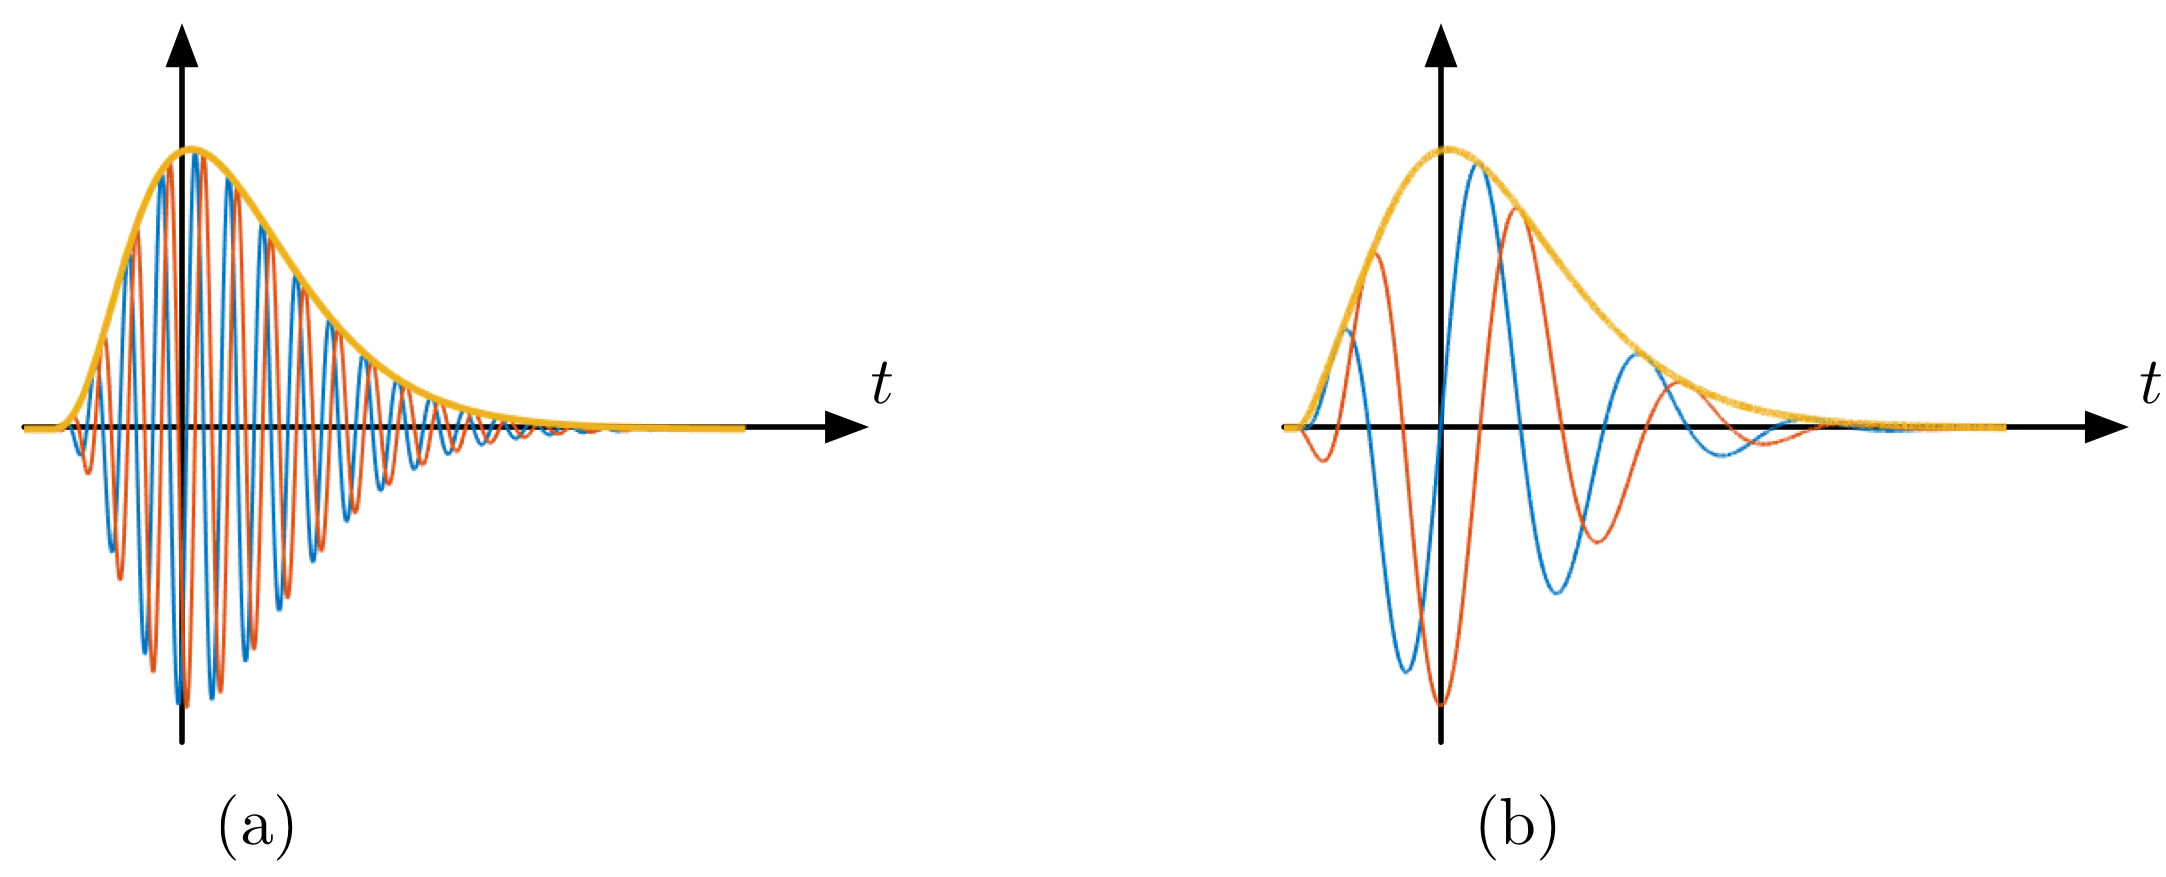
\includegraphics[width=\columnwidth]{gammatones.png}
\caption{
\label{fig:gammatones}
Gammatone wavelets $\psi(t)$ in the time domain with quality factors (a) $Q = 4$ and (b) $Q = 1$. Blue and red oscillations represent the real and imaginary parts. The orange envelope represents the complex modulus.}
\end{center}
\end{figure}

Wavelets
$\boldsymbol{\psi_{\gamma_1}}(t)$ and $\boldsymbol{\psi_{\gamma_2}}(t)$ are designed as fourth-order Gammatone
wavelets with one vanishing moment \cite{Venkitaraman2014}, as shown in Figure \ref{fig:gammatones}.
In the context of auditory scene analysis, the asymmetric envelope of Gammatone wavelets is more biologically plausible than the symmetric, Gaussian-like envelope of the widespread Morlet wavelets.
Indeed, it allows to reproduce two important psychoacoustic effects in the mammalian cochlea: the asymmetry of temporal masking and the asymmetry of spectral masking \cite{Fastl2007}.
Moreover, it should be noted that Gammatone wavelets follow the typical amplitude profile of natural sounds, beginning with a relatively sharp attack and ending with a slower decay.
As such, they can be discovered automatically by unsupervised encoding of natural sounds \cite{Smith2006}.

The next section introduces some techniques in feature design to improve auditory scene classification with scattering coefficients.

\section{Feature design}
Before supervised or unsupervised classification, it is beneficial to process scattering coefficients with feature transformations that improve invariance, normality, or generalization power. 
In this section, we review several ways of achieving these properties, namely binaural data augmentation, feature selection, logarithmic compression, standardization, and temporal integration.
The former has, to the best of our knowledge, not being considered for ASC and is specific to multichannel recordings, whereas the next ones would also apply to many other kinds of data.

\subsection{Feature selection by restricting the frequency range}
In a multivariate time series of descriptors $\mathbf{S}\boldsymbol{x}(t,\gamma)$, some coefficients $\gamma$ may consistently bear negligible information for the task of interest.
This fact may cause the classifier to overfit the training set, especially when the number of features is large and the number of training instances is small, as is the case here.
Selecting features appropriately before the training stage may circumvent this problem.
However, the parameters of the chosen feature selection algorithm are themselves prone to overfitting.
Instead, we adopt the more conservative approach of retaining all coefficients within a certain range of subband indices $\gamma_1$ and $\gamma_2$.
In comparison with adaptive algorithms, the subset of selected features $\gamma$ has a suboptimal statistical relevance, but it is easily interpretable in the realm of audio signal processing, as it is equivalent to a coarse band-pass filtering of $\boldsymbol{x}(t)$ and $\boldsymbol{x_1}(t,\gamma_1)$ over the time dimension $t$.

The conservation equations underlying the physics of sound production constrain the waveform $\boldsymbol{x}(t)$ to be regular in the time domain, that is, to have a polynomial decay in the Fourier domain.
This decay is only made sharper by the specific properties of acoustic environments, especially indoor.
Consequently, the amount of energy in the wavelet subband $\gamma_1$ is roughly inversely proportional to the center frequency $2^{-\gamma_1/Q_1}$.
In the topmost frequencies, this amount is so faint that the corresponding coefficients $\boldsymbol{x_1}(t,\gamma_1)$ and $\boldsymbol{x_2}(t,\gamma_1,\gamma_2)$ no longer bear discriminative information for the classification task at hand.

In the sequel, we evaluate the impact of discarding the scattering coefficients above a certain acoustic frequency $\xi_{1,\max}$, which corresponds to discarding subbands $\gamma_1$ below a certain scale
\begin{equation}
\gamma_{1,\min} =
\left\lfloor Q_1 \log_2 \frac{\xi_1}{\xi_{1,\max}} \right\rceil,
\end{equation}
where $\lfloor \cdot \rceil$ denotes a rounding to the nearest integer.

Reducing the frequency range is an effective way to enhance invariance, widely used in the literature.
For instance, \cite{roma2013} achieved the best performance in the 2013 edition of the DCASE challenge, rely on cepstral descriptors computed up to a cutoff frequency as small as $\xi_{1,\max}  = 900\,\mathrm{Hz}$ instead of the more conventional value of $16\,\mathrm{kHz}$.
 
\subsection{Logarithmic compression}
\label{sec:logcomp}

Many algorithms in pattern recognition, including nearest neighbor classifiers and support vector machines, tend to work best when all features follow a standard normal distribution across all training instances.
Yet, because of the complex modulus nonlinearity, scattering coefficients are nonnegative by design.
It appears empirically that their distribution is skewed towards the right, which means that the tail towards greater values is longer than the tail towards lower values.
However, skewness can be reduced by applying to all coefficients a pointwise concave transformation, \eg logarithmic.
Figure \ref{fig:histograms} shows the distribution of an arbitrarily chosen scattering coefficient over the DCASE 2013 dataset, before and after logarithmic compression.


\begin{figure}
\begin{center}
%\begin{tikzpicture}
%\useasboundingbox[red] (-0.25, -0.5) rectangle (8.25, 2);
%\node[anchor=south west,inner sep=0] at (-0.36, 0) {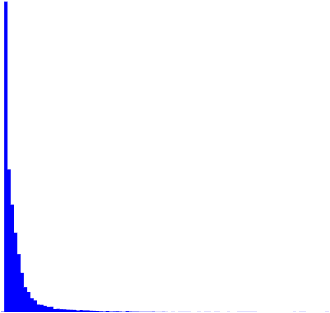
\includegraphics[height=2cm,width=5cm]{feature_histogram.png}};
%\node (histlabel1) at (2.3, 0.01) {$\mathbf{S}\boldsymbol{x}(\gamma)$};
%\draw[-{Latex[length=2mm]}] (-0.3, 0.01) -- (histlabel1);
%\draw[-{Latex[length=2mm]}] (-0.3, 0.01) -- (-0.3, 2.5);
%\node at (0.8, -0.35) {(a)};
%\node (histlabel2) at (7.6, 0.01) {$\log \mathbf{S}\boldsymbol{x}(\gamma)$};
%\node[anchor=south west,inner sep=0] at (3.45, 0) {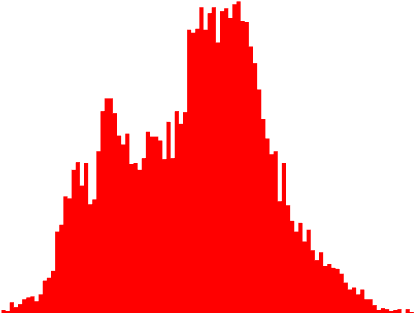
\includegraphics[height=2cm,width=3cm]{feature_histogram_logcompressed.png}};
%\draw[-{Latex[length=2mm]}] (3.2, 0.01) -- (histlabel2);
%\draw[-{Latex[length=2mm]}] (4.9, 0.01) -- (4.9, 2.5);
%\node at (4.9, -0.35) {(b)};
%\end{tikzpicture}
\caption{
\label{fig:histograms}
Histogram of values taken by the first-order scattering coefficient $\mathbf{S}\boldsymbol{x}(\gamma)$, corresponding to a center acoustic frequency of $302\,\mathrm{Hz}$,
(a) before and (b) after logarithmic compression.}
\end{center}
\end{figure}


The application of the pointwise logarithm to magnitude spectra is ubiquitous in audio signal processing.
Indeed, it is corroborated by the Weber-Fechner law in psychoacoustics, which states that the sensation of loudness is roughly proportional to the logarithm of the acoustic pressure.
We must also recall that the measured amplitude of sound sources often decays polynomially with the distance to the binaural microphone, which is a spurious factor of variability to the task of auditory scene classification.
Logarithmic compression can linearize this dependency, which arguably facilitates the construction of a powerful invariant at the classifier stage.

Given a task of musical genre recognition, \cite{Anden2014} has advocated for the renormalization of second-order scattering coefficients $\mathbf{S_2}\boldsymbol{x}(t,\gamma_1,\gamma_2)$ by the corresponding first-order scattering coefficients $\mathbf{S_1}\boldsymbol{x}(t,\gamma_1)$, as it provably decorrelates the amplitudes of their activations.
Interestingly, taking the logarithm of renormalized coefficients would yield
\begin{equation}
\log \dfrac{\mathbf{S_2}\boldsymbol{x}(t,\gamma_1,\gamma_2)}{\mathbf{S_1}\boldsymbol{x}(t,\gamma_1)} =
\log \mathbf{S_2}\boldsymbol{x}(t, \gamma_1, \gamma_2) -
\log \mathbf{S_1}\boldsymbol{x}(t, \gamma_1),
\end{equation}
\ie a linear combination of the logarithms of first- and second-order coefficients.
Therefore, the theoretical insight brought by \cite{Anden2014} in favor of renormalized scattering also applies to log-scattering up to a linear transformation in feature space, to which affine classifiers are not sensitive.

\subsection{Early \vs late temporal integration}
\label{sec:eili}

Owing to the scarcity of salient events in many natural scenes,
fine-grained classification is only made
possible by integrating signal information over a long temporal context.
Indeed, whereas a few seconds are often sufficient to recognize a speaker,
a musical instrument, or a genre, it may require up to 30 seconds
to disambiguate two classes auditory scenes which share part of their semantic content, \eg a train from a subway station or a quiet street from a park.
Depending on whether aggregation is performed in feature space or in decision space, the corresponding method is referred to as early or late integration.

A straightforward application of early integration consists in summarizing the multivariate time series of scattering coefficients over the full duration of the auditory scene, by retaining their average values only.
Going back to the definition of the scattering transform given in section \ref{sec:scattering}, this is equivalent to increasing the support $T$ of the low-pass filter $\boldsymbol{\phi}(t)$ up to infinity. With a slight abuse of notation, we denote by
\begin{equation}
\mathbf{S}\boldsymbol{x}(\gamma) =
\int_{-\infty}^{+\infty} \mathbf{S}\boldsymbol{x}(t,\gamma)\;\mathrm{d}t
\end{equation}
the summarized features.

Conversely, a late integration scheme relies on probabilistic estimates over short-term windows of length $T$, which are subsequently aggregated to produce a final decision
\begin{equation}
\hat{y} = \arg \max_{y} \rho\Big(\big\{ \mathbb{P}\left[y \,\vert\, \mathbf{S}\boldsymbol{x}(t,\gamma) \right] \big\}_{t} \Big),
\end{equation}
where $\hat{y}$ is the estimated class label and $\rho$ is a reduction function, such as sum, product, or majority vote \cite{Kittler1998}.

The principal drawback of early integration is that it drastically reduces the number of training instances at the classifier stage, down to one per auditory scene -- if data augmentation is not considered.
In the context of the DCASE 2013 dataset, this corresponds to merely $8$ training instances per class, and $80$ instances overall, hence an increase in variance in statistical estimation and a risk of overfitting.
On the contrary, a late integration scheme for $T=188\textrm{ ms}$ would yield $128$ instances per auditory scene, resulting in $10240$ instances overall.
However, many of these instances may be silent or lack any salient properties of the class they are assigned to, hence an increase in bias and a risk of underfitting.
In short, early and late integration methods lie at opposite ends of the bias-versus-variance statistical tradeoff. We refer to \cite{Joder2009} for a comprehensive review of this problematic in the context of musical instrument recognition.

\subsection{Standardization}
\label{sec:stand}

Let $\mathbf{S}\boldsymbol{X}(\gamma,n)$ be a dataset, where the indices $\gamma$ and $n$ respectively denotes features and examples.
It is commonly acknowledged that support vector machines should be trained on scaled features with null mean and unit variance, so as to avoid mismatch in numeric ranges.
This operation may also help making the dataset linearly separable in feature space.
To standardize $\mathbf{S}\boldsymbol{X}(\gamma,n)$, we apply the affine transformation
\begin{equation}
\widetilde{\mathbf{S}}\boldsymbol{X}(\gamma, n) =
\dfrac{ \mathbf{S}\boldsymbol{X}(\gamma, n) -
\mathbb{E}[ \mathbf{S}\boldsymbol{X}](\gamma)}{\sigma[ \mathbf{S}\boldsymbol{X}](\gamma)}
\end{equation}
where $\mathbb{E}[ \mathbf{S}\boldsymbol{X}](\gamma) = \frac{1}{N} \sum_{n=1}^{N} \mathbf{S}\boldsymbol{X}(\gamma,n)$ is the expected value of $\mathbf{S}\boldsymbol{X}(\gamma,n)$ and
\begin{equation}
\sigma[\mathbf{S}\boldsymbol{X}] (\gamma) =
\sqrt{\frac{1}{N-1} \sum_{n=1}^{N}
\left( \mathbf{S}\boldsymbol{X}(\gamma,n) - \mathbb{E}[\mathbf{S}\boldsymbol{X}] \right)^2}
\end{equation}
 is the sample standard deviation.
 
 The vectors $\mathbb{E}[\mathbf{S}\boldsymbol{X}(\gamma)]$ and $\sigma[\mathbf{S}\boldsymbol{X}](\gamma)$ are estimated from the training set only, and the same affine transformation is subsequently applied to all samples in the training set and the test set.
 
The next section discusses adaptive methods for the temporal integration of scattering coefficients in an unsupervised setting.

\section{Object-based modeling of the scene}
\label{sec:object}

%As part of the aforementioned research areas and applications, the emerging field of \emph{Acoustic Scene Analysis} (also called \emph{Sound Scene Analysis}) \cite{Stowell15} aims to develop approaches and systems for the automatic analysis of environmental sounds and soundscapes (originating both from urban or nature environments). While research methodologies in related fields such as Automatic Speech Recognition (ASR) \cite{Rabiner93} and Music Information Retrieval (MIR) \cite{Muller07} are now well established, research addressing Acoustic Scene Analysis remains relatively young. 

%From a data processing point of view, a holistic scheme, such as the bag-of-frame approach \cite{aucouturier2007bag}, has a simplicity, but clearly face poor performance on realistic conditions \cite{lagrange:hal-01082501}. 

\gl{vincent, un petit mot pour motiver le fait que le scattering est un bon outil pour separer les evenements peuplant une scène sonore ?}. 

As discussed in Section \ref{sec:motivations}, several outcomes in sound perception encourage us to evaluate the validity of an object-based representation of the scene for predicting high-level properties. Though, a perfect knowledge of which event occurred at a given time is not feasible. In this paper, we thus focus on a simple quantization scheme in order to favor genericity, implemented using a clustering approach where coherent regions of the scene are identified.

One should note that this quantization approach differs from unsupervised learning schemes such as the ones studied in \cite{bisot2016acoustic} that performs some variances estimates over the whole dataset and not solely on each scene, and reproject each scene in the resulting enhanced features space. Here, the aim of this process is to better balance the impact of salient events and texture like sounds on final decision by considering several ways of computing the similarity between scenes based on their centroids :

\begin{itemize}
\item \emph{ob-closest} (ob-c): the similarity between two scenes is equal to the largest similarity between their centroids.
\item \emph{ob-averaged} (ob-a): the similarity between two scenes is equal to the average of their centroids similarities.
\item \emph{ob-weighted} (ob-w): for each scene, each centroid is weighted according to the number of frames belonging to its cluster.
\end{itemize}

The similarity between two centroids $c_i$ and $c_j$ is computed using a radial basis function (RBF) kernel $K^c$ combined with the local scaling method proposed in \cite{selfTuneManor2004}:
\begin{equation}
\label{eq:kc}
K^c_{ij} = exp\left( - \dfrac{\Vert c_i - c_j \Vert^2}{\Vert c_i - c_N \Vert \Vert c_j - c_N \Vert} \right) 
\end{equation}

where $c_N$ is the $N^{\mathrm{th}}$ nearest neihgbor of the centroid $c_i$, and $\Vert \cdot \Vert$ denotes the Euclidean norm. 

Compared to the closest or averaged approach, the  weighted similarity between two scenes takes into account both the centroids similarities and the clusters weights. Each scene $s_u$ is described by a signature $S_u$ of $m$ clusters ($S_u=\lbrace(c_1^u,w_1^u),\ldots,(c_m^u,w_m^u)\rbrace$), with $c_i^u$ and $w_i^u$ being the centroid and the weight of the $i$th cluster of the scene $s_u$ respectively. 

To compute the distance between two signatures $S_u$ and $S_v$, we use a variant version of the Earth Moving Distance ($EMD$), known as $\widehat{EMD}$ and introduced in \cite{pele2008linear}. $EMD$ is a cross-bin histogram distance, widely used in computer vision \cite{zhang2007local}, which compute the minimal cost to be paid to transform one histogram into the other. The advantage of using the $EMD$ is that it does not require bins to be aligned. The alignment problem is solved by using a ``\,ground distance\,'', which is the distance between the bins representatives of the two histograms. In our case, the histograms are the cluster weights $w$, and the bins representative the cluster centroids $c$.

$\widehat{EMD}$ is a variant version of the $EMD$ adapted for non-normalized histograms. To compute the $\widehat{EMD}$, we use the implementation proposed in \cite{pele2009fast}. Given two signatures $S_u$ and $S_v$, the $\widehat{EMD}$ is computed by solving the following linear programming problem:

\begin{equation}
\begin{split}
\widehat{EMD}(S_u,S_v) &=( \min\limits_{\lbrace f_{ij}\rbrace} \sum\limits_{i,j} f_{ij}D_{ij} )  \\ 
&+ \mid \sum\limits_{i} w_i^u - \sum\limits_{j} w_j^v  \mid \alpha \max\limits_{i,j}\lbrace  D_{ij}\rbrace
\end{split}
\end{equation}

\begin{equation*}
s.t. \quad f_{ij}\geq0 \quad \sum\limits_{j} f_{ij} \leq w_i^u \quad \sum\limits_{i} f_{ij} \leq w_j^v 
\end{equation*}

\begin{equation*}
\sum\limits_{i,j}f_{ij} = \min( \sum\limits_{i} w_i^u ,\sum\limits_{j} w_j^v )
\end{equation*}

where $\lbrace f_{ij} \rbrace$ is the optimal flow between the cluster weights $w_i^u$ and $w_j^v$, that is, the amount transported from the $i$th bin to ``\,supply to the demand\,'' of the $j$th bin. $D_{ij}$ is the ground distance between the centroids $c_i^u$ and $c_j^v$, and is computed from the kernel $K^c$:

\begin{equation*}
D_{ij}=1-K^{c(uv)}_{ij}
\end{equation*}

with $K^{c(uv)}$ being the slice of $K^{c}$ containing the pairwise similarities between the centroids sets $c^u$ and $c^v$ of the scenes $s_u$ and $s_v$ respectively. As suggested in \cite{pele2009fast}, we set the $\alpha$ parameter to one.

To get the final similarity measure between the scenes $s_u$ and $s_v$, an extended Gaussian kernels $K^s$ \cite{chapelle1999support,jing2003support} is computed:

\begin{equation}
\label{eq:ks}
K_{uv}^s = exp\left( - \dfrac{\widehat{EMD}(S_u,S_v)}{A} \right) \\
\end{equation}

with $A$ a scaling parameter, set to the mean value of the $\widehat{EMD}$ between all the scenes. The resulting kernel $K^s$ is called an EMD kernel, and it has to be noted that there is no proof that such kernel is positive definite. \\

%\ml{Grégoire : if the matrix is not psd, then this is NOT a kernel, reformulate}

\section{Experiments}
\label{sec:experiments}

\subsection{Feature design}

Experiments are carried out using temporal-scattering coefficients as well as Mel Frequency Cesptral Coefficients (MFCCs) as features. For the temporal-scattering, each scene is described by 128 vectors of scattering coefficients, with half-overlapping windows $\boldsymbol{\phi}(t)$ of duration $T=188\,\mathrm{ms}$. Experiments are conducted with and without the logarithmic compression (see Section \ref{sec:logcomp}).

Different sets of parameters were tested to compute the MFCCs. Results here are only reported for the best setting. 40 MFCCs (including the first energy coefficient) are computed for windows of 50ms and hops of 25ms, with a full frequency range. This setting gives us 600 feature vectors per scenes. It has been reported that classifying the full set of frames directly may not be the best approach \cite{rakotomamonjy2015histogram}. In order to reduce the data dimensionality, a pooling step is performed on the MFCCs vectors: each set of MFCCs vectors is divided into $n$ non-overlapping $t$-seconds long "texture" windows. Each $n$ texture windows are then averaged over time. As the \emph{ob} approaches involve a clustering step, it is desirable to ensure that each scene is described by circa the same number of vectors prior to the clustering step, for both the temporal-scattering and the MFCCs. Thus, $t$ is set to 250ms, resulting in 120 MFCCs texture windows per scene. 

\subsection{Methods}

The influence of the temporal-scattering transform and the \emph{ob} approaches are assessed in an unsupervised setting (\emph{i.e.} ASSR) and in a supervised setting (\emph{i.e.} ASC). 

For the ASSR setting, evaluation is performed on the private dataset of the DCASE 2013 challenge. The metric used is the precision at rank $k$ ($p@k$), which is the  average  number  of  items  of  the  same  class among the $k$ closest items averaged for all possible seed items. The $p@k$ is computed for $k=[1,\ldots,9]$, $9$ being the number of elements that are of the same class than the seed item. Note that a $p@1$ is equivalent to an accuracy computed based on the labels of the 1st nearest neighbors of the items to classify. For each experimental setting, we only report the results obtained with the sets of parameters, \emph{i.e.} the number of clusters $m$ for the \emph{ob} approaches and the scaling parameter $N$ of the RBF kernels (see Eq. \ref{eq:kc}) leading to the best $p@9$.
 
For the ASC setting, the systems are evaluated  with five-fold  stratified cross validation on the private dataset of the DCASE 2013 challenge. The folds are identical to those used in the original challenge. Optimal parameters (see above) are this time learned on the public dataset of the DCASE 2013 challenge, using five-fold  stratified cross validation as well. Clustering is done using an enhanced version of the popular K-means algorithm known as $K$-means$++$ \cite{arthur2007k}, which differs from k-means method in terms of selection of starting points. 

The \emph{ob} approaches are compared to commonly used approaches using an early integration strategy (\emph{early}) for the ASSR setting, and both an early and a late integration (\emph{late}) strategy for the ASC setting (see Section \ref{sec:eili}). In thsi context early integration refers to an averaging of the features and late integration refers to a majority voting of the predictions.

As most of the 2013 DCASE challenge participants did, a Support Vector Machine (SVM), which is a large-margin binary discriminators with tunable regularization of misclassified examples, is used as classifier for the ASC setting. The parameter $C$ is here set to one.

For the \emph{ob} approaches, we use the precomputed kernels described in Section \ref{sec:object}. For both the \emph{early} and \emph{late} approaches, a linear kernel as well as a RBF kernel are used. As for the \emph{ob} approaches, the RBF kernel is scaled locally using the method proposed in \cite{selfTuneManor2004}. All feature vectors, being frames, texture windows or centroids are standardized prior to be given to the classifier. The standardization is computed with respect to the train/test set splits of the cross validation scheme (see Section \ref{sec:stand}).

\section{Results \label{sec:results}}

\begin{figure}
\begin{center}
\includegraphics[width=8cm]{gfx/unsupervised_test3.eps}
\caption{ASSR: $p@k$ obtained for MFCCs and scattering with logarithmic compression}
\label{fig:ASS_1}
\end{center}
\end{figure}

\begin{figure}
\begin{center}
\includegraphics[width=8cm]{gfx/unsupervised_test2.eps}
\caption{ASSR: $p@k$ obtained for scattering with and without logarithmic compression (w/o log)}
\label{fig:ASS_2}
\end{center}
\end{figure}

\subsection{Acoustic Scene Similarity Retrieval}

This section present evaluation results for the ASSR settings. The $p@k$ for different settings are showed in the Figures~\ref{fig:ASS_1} and \ref{fig:ASS_2}.

\subsection*{MFCC \vs scattering transform}

Irrespective of the rank $k$ considered, best result is achieved for the scattering transform with logarithmic compression using the \emph{ob-c} approach. Overall, log-compressed scattering coefficients systematically outperform MFCCs.

\subsection*{Object-based \vs early integration}

For the scattering, \emph{ob-c} and \emph{ob-w} outperform \emph{early}, thus confirming the benefits of using an object-based representation to refine the similarity measures between the scenes. However, it is worth noticing that \emph{ob-a} perform equivalently to \emph{early}, which shows that the discriminant information is not carried by all the centroids. To take advantage of an object-based representation, a selection step has to be run on the representatives of the scenes. Furthermore It appears that \emph{ob-c} is be able to better characterize the classes than \emph{ob-w}. This last observation suggests that weighted a centroid according to the number of frames belonging to it may prove to be a limited solution. Indeed, nothing a priori indicates that the discriminant information between two scenes lays within the majority of their frames. On the contrary, two similar environments may shared a lot of similar sound sources.

For the MFCCs, there is no clear evidence that the \emph{ob} approaches improve the results.

\subsection*{Role of logarithmic compression}

Outcomes for the scattering with and without logarithmic compression are showed in Figure~\ref{fig:ASS_2}. It can be seen that the logarithmic compression strongly improves the results, specially for the \emph{ob} approaches, which perform lesser than \emph{early} without the logarithmic compression. \gl{une idée du pourquoi ?}

\subsection{Acoustic Scene Classification}


\begin{figure}
\begin{center}
\includegraphics[width=\columnwidth]{gfx/supervised_rbf_test3.eps}
\caption{...}
\end{center}
\end{figure}

\begin{table}
\begin{center}
\begin{tabular}{llll}
             & MFCCs         & scattering & log-scattering  \\
             \hline
early (linear)  & 54 (20)       & 62 (6)  & 66 (11)     \\
early (RBF)     & 47 (16)       & 56 (7)  & 63 (6)    \\
late (linear)  & 60  (9)       & 70 (8)  & 75 (5)   \\
late (RBF)     & 68 (10)       & 73 (8)  & 78 (6)   \\
\end{tabular}
\caption{ASC: Accuracies for the best settings}
\end{center}
\end{table}

MFCC \vs scattering

Object-based \vs early/late integration

Role of logarithmic compression

\vl{Results: DCASE 2016}

\section{Conclusion}

In this paper, the benefit of considering 1) the scattering transform for building discriminant features and 2) unsupervised clustering for the modeling of large time span environmental acoustic scenes.
This leads to improvement both for the ASSR and ASC tasks.

Abstracting the scene as a reduced set of exemplars with adapted similarity strategies allows us to improve ASSR performance when the BOF approaches based on GMMs fails with reference to an early integration scheme. Those results advocate for a hierarchical model of the scene, where small time scale structure -- \ie below a second -- shall be decorrelated using ca onvolutional network such as in the scattering transform, whereas larger time scales -- \ie over a second -- structure shall be modeled as adaptive aggregates that can be identified in the time domain in an unsupervised setting and in the features domain in the supervised case, provided that the dimensionality is sufficiently high.

This assertion shall be studied further in future work by considering more complex convolutional networks, larger databases and more diverse application scenarios, such as pleasantness prediction \cite{lafaySoundscapePilot, lafay:hal-01111782} or ecoacoustics tasks.

\bibliographystyle{unsrt}
\bibliography{biblio}

% biography section
% 
% If you have an EPS/PDF photo (graphicx package needed) extra braces are
% needed around the contents of the optional argument to biography to prevent
% the LaTeX parser from getting confused when it sees the complicated
% \includegraphics command within an optional argument. (You could create
% your own custom macro containing the \includegraphics command to make things
% simpler here.)
%\begin{IEEEbiography}[{\includegraphics[width=1in,height=1.25in,clip,keepaspectratio]{mshell}}]{Michael Shell}
% or if you just want to reserve a space for a photo:

%\begin{IEEEbiography}{Mathieu Lagrange}
%Biography text here.
%\end{IEEEbiography}

% if you will not have a photo at all:
%\begin{IEEEbiographynophoto}{John Doe}
%Biography text here.
%\end{IEEEbiographynophoto}

% insert where needed to balance the two columns on the last page with
% biographies
%\newpage

%\begin{IEEEbiographynophoto}{Jane Doe}
%Biography text here.
%\end{IEEEbiographynophoto}

% You can push biographies down or up by placing
% a \vfill before or after them. The appropriate
% use of \vfill depends on what kind of text is
% on the last page and whether or not the columns
% are being equalized.

%\vfill

% Can be used to pull up biographies so that the bottom of the last one
% is flush with the other column.
%\enlargethispage{-5in}



% that's all folks
\end{document}


